% --------------------------------------------------------------------
% Anexos -------------------------------------------------------------

% Código para agregar el informe académico en formato PDF ------------
% 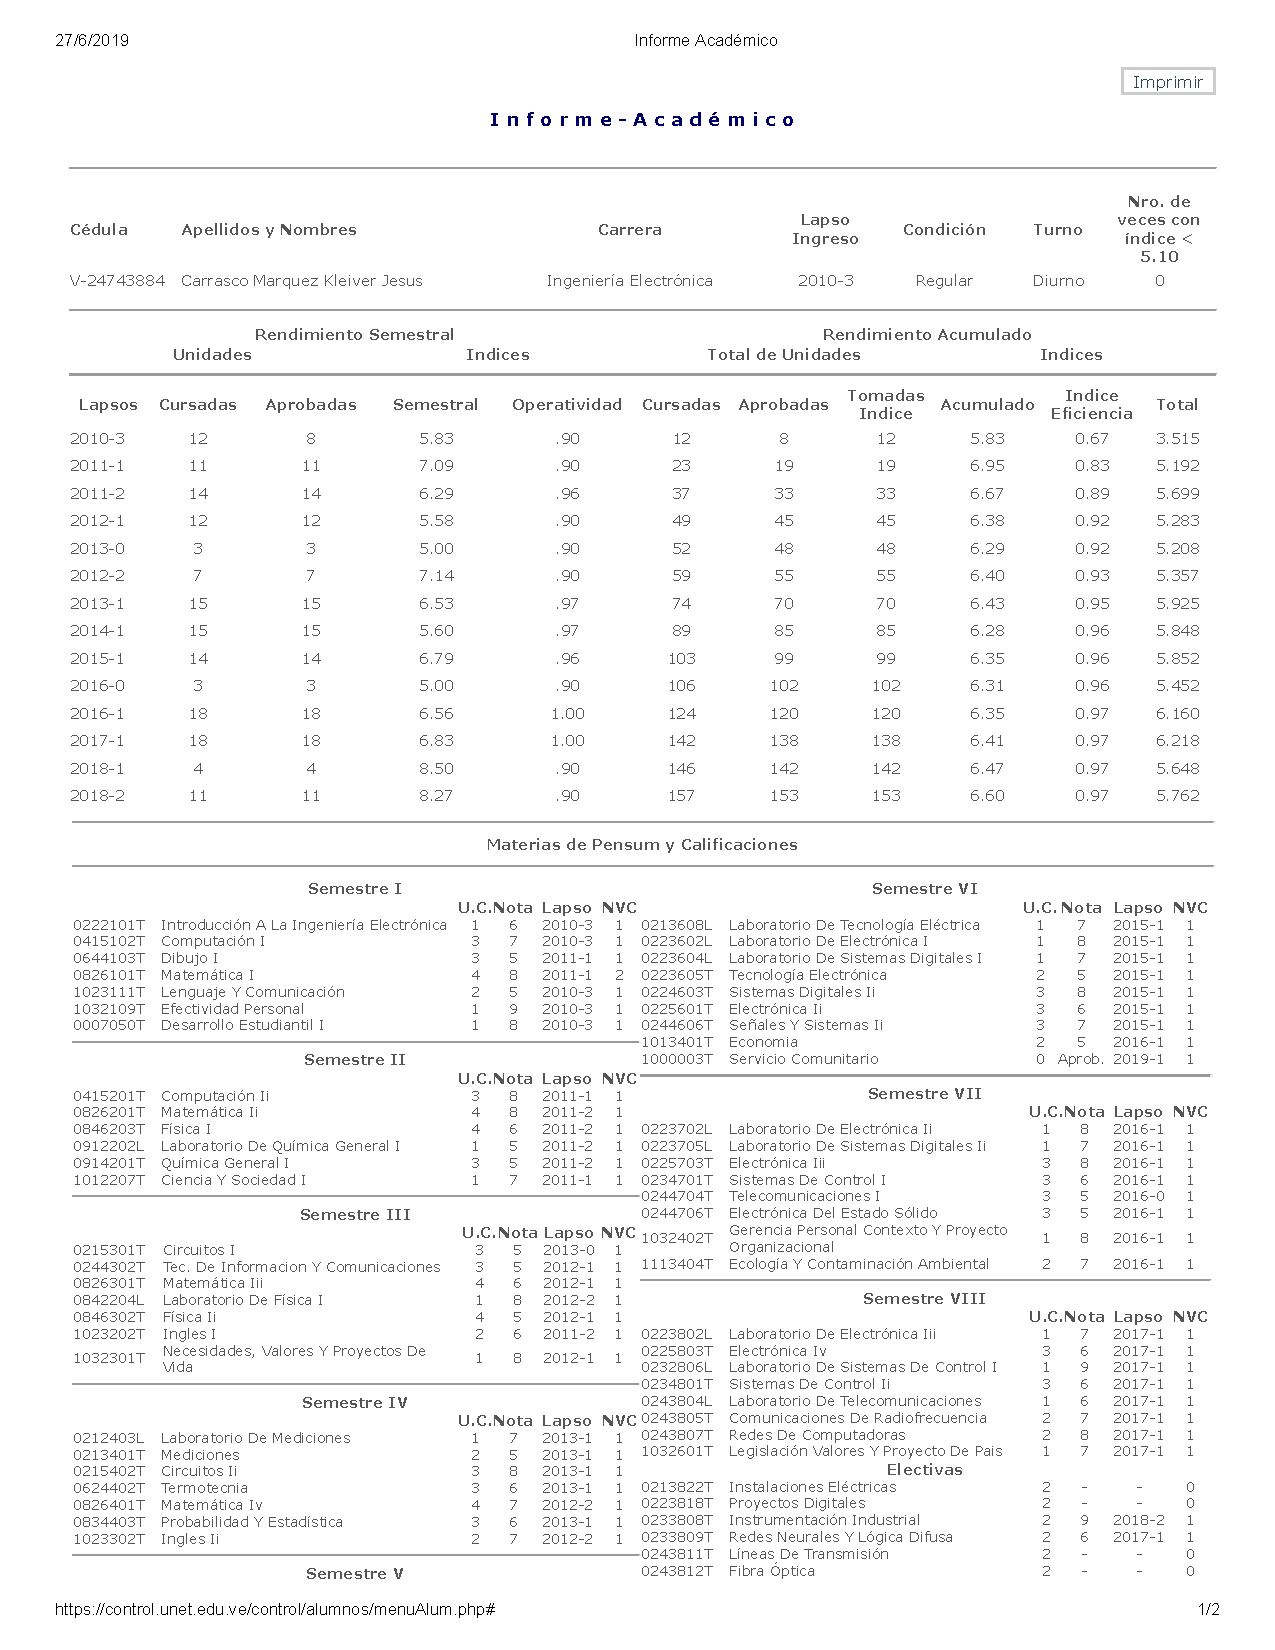
\includepdf[scale=0.7,pages=1,pagecommand={\AgregarAnexo{Informe académico}}, 
% addtotoc={1, chapter, 0,\bfseries\uppercase{Anexos}, pdf:informe}]{imagenes/informeAcademico}
% \includepdf[scale=0.7,pages=2, pagecommand={}]{imagenes/informeAcademico}
% --------------------------------------------------------------------
% Nota: Si se utiliza este código se deben comentar:
% \newpage
% \phantomsection
% \addcontentsline{toc}{chapter}{Anexos}
% --------------------------------------------------------------------

\newpage                                % Comentar si se incluye
\phantomsection                         % primero un pdf
\addcontentsline{toc}{chapter}{Anexos}  % Para evitar problemas TOC

% Para agregar anexos a la tesis
\AgregarAnexo{Titulo del anexo}
    \blindtext

\AgregarAnexo{Titulo de otro anexo}
    \blindtext